\section[Kellerautomaten (\acs*{PDA})]{Kellerautomaten \quad\normalfont\normalsize \acf{PDA}}
\newcommand{\ConfRel}{\rhd}
\newcommand{\Zinit}{Z^\mathsf{init}}
\newcommand{\K}{\mathcal{K}}
\newcommand{\el}[3]{{\color{red!70!black}#1};{\color{blue!70!black}#2};{\color{blue!70!black}#3}}

Die im letzten Kapitel vorstellten kontextfreien Sprachen können wir bisher nur mit Hilfe von kontextfreien Grammatiken darstellen.
Für die regulären Sprachen aus Kapitel~\ref{sec:reglang} haben wir dagegen mit DEAs, NEAs, $\Eps$-NEAs, regulären Ausdrücken und regulären Grammatiken verschiedene Darstellungsformen kennengelernt.
Die Automaten hatten dabei für uns einen besonderen Reiz, da diese Darstellungsform Ähnlichkeiten mit Computern hat.
In diesem Kapitel werden wir nun den Kellerautomaten, ein Automatenmodell für die kontextfreien Sprachen, kennenlernen.

Ein Kellerautomat ist im wesentlichen ein $\Eps$-NEA, der um einen Stapelspeicher mit unbeschränkter Kapazität erweitert wurde.

Bei jedem Zustandsübergang darf der Kellerautomat das oberste Element des Stapelspeichers inspizieren und durch eine (potentiell leere) Sequenz von Elementen ersetzen.
Der Automat darf dabei die Entscheidung über den Folgezustand vom inspizierten Element abhängig machen.
Zu Beginn liegt genau ein Element, das \emph{Kellerbodensymbol}, auf dem Stapelspeicher.

Der Kellerautomat unterscheidet sich noch in einem weiteren Detail vom $\Eps$-NEA:
Es gibt keine akzeptierende Zustände. 
Der Kellerautomat akzeptiert stattdessen, wenn am Ende eines Zustandsübergangs das Eingabewort komplett gelesen wurde
und der Stapelspeicher leer ist.

Analog zu endlichen Automaten können wir auch Kellerautomaten mit Hilfe eines Zustandsdiagramms beschreiben.
Ein Beispiel ist in \autoref{pdaEvenPalindrome} dargestellt.
Alle Transitionen sind mit einem Tripel beschriftet. 
Die erste Komponente des Tripels ist dabei das gelesene Zeichen der Eingabe,
die zweite Komponente ist das vom Stapelspeicher genommene Element und
die dritte Komponente ist die Sequenz, die auf den Stapelspeicher gelegt wird.

\begin{figure}[H]\centering
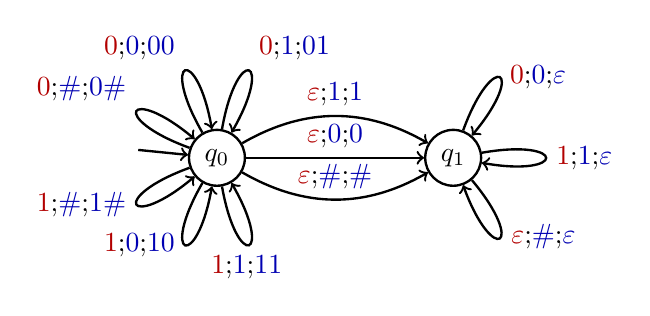
\begin{tikzpicture}[line width=0.3mm,
tape/.style={draw, node distance=0mm, minimum size=6mm, text=red!70!black, font=\bf},
tapeend/.style={node distance=0mm, minimum size=6mm, text=red!70!black, font=\bf},
stack/.style={draw=blue!50!black, node distance=0mm, minimum size=6mm, text=blue!70!black, font=\bf}
]

% \node (rect) at (0,0) [draw, rounded corners=2, fill=lightgray!20,thick,minimum width=9cm,minimum height=4cm] {};
 
 \node[circle,draw] (q1) at (-1.5,0) {$q_0$};
 \node[circle,draw] (q2) at (1.5,0) {$q_1$};
 
 
 \draw[->] (-2.5,0.1) to  (q1) ;
 
 \draw[->] (q1) edge node[auto] {\el{$\varepsilon$}{0}{0}} (q2) ;
 \draw[->, bend left] (q1) edge node[auto] {\el{$\varepsilon$}{1}{1}} (q2) ;
 \draw[->, bend right] (q1) edge node[auto] {\el{$\varepsilon$}{\#}{\#}} (q2) ;
 
 \draw[->,in=140, out=160, looseness=22, pos=0.50] (q1) edge node[auto] {\el{0}{\#}{0\#}} (q1) ;
 \draw[->,in=100, out=120, looseness=22, pos=0.50] (q1) edge node[auto] {\el{0}{0}{00}} (q1) ;
 \draw[->,in=60, out=80, looseness=22, pos=0.50] (q1) edge node[auto] {\el{0}{1}{01}} (q1) ;
 
 \draw[->,in=220, out=200, looseness=22, pos=0.50] (q1) edge node[left] {\el{1}{\#}{1\#}} (q1) ;
 \draw[->,in=260, out=240, looseness=22, pos=0.50] (q1) edge node[left] {\el{1}{0}{10}} (q1) ;
 \draw[->,in=300, out=280, looseness=22, pos=0.45] (q1) edge node[below] {\el{1}{1}{11}} (q1) ;
 

 \draw[->,in=50, out=70, looseness=22, pos=0.50] (q2) edge node[right] {\el{0}{0}{$\varepsilon$}} (q2) ;
 \draw[->,in=-10, out=10, looseness=22, pos=0.50] (q2) edge node[right] {\el{1}{1}{$\varepsilon$}} (q2) ;
 \draw[->,in=-70, out=-50, looseness=22, pos=0.45] (q2) edge node[right] {\el{$\varepsilon$}{\#}{$\varepsilon$}} (q2) ;
\end{tikzpicture}
	\caption{Zustandsdiagramm eines Kellerautomaten}
	\label{pdaEvenPalindrome}
\end{figure}

Der in \autoref{pdaEvenPalindrome} dargestellte Kellerautomat akzeptiert die Sprache $L=\{ww^R\mid w\in\{0,1\}\}$
und verwendet das Zeichen $\#$ als Kellerbodensymbol.
In Zustand $q_0$ wird für jedes Eingabezeichen das entsprechende Symbol auf den Stapelspeicher gelegt.
Zu jedem Zeitpunkt kann der Automat nichtdeterministisch (mit Hilfe einer $\Eps$-Transition) in den Zustand $q_1$ wechseln.
Diese Transition sollte genau bei der Hälfte des Eingabeworts genommen werden.
In Zustand $q_1$ vergleicht der Automat sukzessive die verbleibenden Eingabesymbole mit dem Inhalt des Stapelspeichers.
Nur bei Übereinstimmung wird der Stapelspeicher bis zum Kellerbodensymbol geleert.
Falls nur noch das Kellerbodensymbol auf dem Stapelspeicher liegt, kann der Automat dieses mit der Transition "`$\Eps;\#;\Eps$"' entfernen und die Eingabe akzeptieren.

Auf Englisch heißen Kellerautomaten \emph{pushdown automata} und wir werden die Abkürzung \ac{PDA} für Kellerautomaten verwenden. 
In diesem Kapitel befassen wir uns zunächst nur mit nichtdeterministischen Kellerautomaten und definieren diese formal wie folgt.


\begin{Def}[name={[NPDA]}]
        Ein \ac{NPDA}\footnote{Englisch: Nondeterministic Pushdown Automaton} ist ein 6-Tupel 
        $$(\Sigma,Q,\Gamma,\qinit,\Zinit,\delta).$$
        Dabei ist
        \begin{itemize}
		\item $\Sigma$ ein Alphabet, das wir auch \emph{Eingabealphabet} nennen,
                \item $Q$ eine endliche Menge, deren Elemente wir \emph{Zustände} nennen,
                \item $\Gamma$ ein Alphabet, das wir auch \emph{Kelleralphabet} nennen,
                \item $\qinit\in Q$ ein Zustand, den wir Startzustand nennen,
                \item $\Zinit\in\Gamma$ ein Zeichen, das wir \emph{Kellerbodensymbol} nennen,
                \item $\delta: Q\x(\Sigma\cup\{\Eps\})\x\Gamma \-> \mathcal{P}(Q\x\Gamma^*)$ eine Funktion, die wir \emph{Transitionsfunktion} nennen. \qedhere
        \end{itemize}
\end{Def}

\begin{Bsp}
\label{bsp:pda-wwr}
Wir beschreiben den in \autoref{pdaEvenPalindrome} abgebildeten Kellerautomaten formal wie folgt.
        \begin{align}
                \Sigma &= \{0,1\} &\qquad&\text{Eingabealphabet} \notag\\
                \Gamma &= \{0,1,\#\} &&\text{Kelleralphabet} \notag\\
                Q &= \{q_0,q_1\} &&\#\,\hat=\,\text{Kellerbodensymbol} \notag\\
                \delta(q_0,a,Z) &= \{(q_0,aZ) \}&& a\in\{0,1\},Z\in\Gamma\\
                \delta(q_0,\Eps,Z) &= \{(q_1,Z)\} \label{eq:5.2}\\
                \delta(q_1,a,a) &= \{(q_1,\Eps)\}\\
                \delta(q_1,\Eps,\#) &= \{(q_1,\Eps)\}
        \end{align}
Hat die graphische Darstellung eines Kellerautomaten sehr viele Transitionen müssen wir diese nicht alle explizit Zeichnen.
Statt dessen können wir auch wie in \autoref{pdaEvenPalindromeNotEplicit}
Variablen verwenden um mehrere Transitionen zusammenzufassen.
        
\begin{figure}[H]\centering
   \begin{center}
  \begin{tikzpicture}[node distance = 3cm]
    \node[state] (0) at (0,0) {$q_0$};
    \node[node distance = 1cm, left of = 0] (start) {};
    \node[state, right of = 0] (1) {$q_1$};

    \draw[->] (start) to (0);
    \draw[->, loop above] (0) to node{$a;Z;aZ$} (0);
    \draw[->] (0) to node[auto]{$\Eps;Z;Z$} (1);
    \draw[->, loop above] (1) to node[auto]{$a;a;\Eps$} (1);
    \draw[->, loop right] (1) to node[auto]{$\Eps;\#;\Eps$} (1);
  \end{tikzpicture}
  $a\in\{0,1\}, Z\in\Gamma$
\end{center}
	\caption{Zustandsdiagramm der Kellerautomaten aus \autoref{pdaEvenPalindrome}. 
	Statt alle Transitionen explizit zu zeichnen verwenden wir die Variablen $a$ und $Z$ um eine Menge von Transitionen durch eine einzige Kante zu repräsentieren. }
	\label{pdaEvenPalindromeNotEplicit}
\end{figure}
\end{Bsp}


Im Weiteren sei $\K=(\Sigma,Q,\Gamma,\qinit,\Zinit,\delta)$ ein \ac{NPDA}.
\begin{Def}[name={[Menge der Konfigurationen eines \acs*{NPDA}]}]
        Die Menge der \emph{Konfigurationen} von $\K$ ist $\Konf(\K) = Q\x\Sigma^*\x\Gamma^*$.\\
        Die \emph{Schrittrelation} von $\K$
  \begin{displaymath}
    \mathop{\ConfRel} \subseteq \Konf(\K) \times \Konf(\K) 
  \end{displaymath}
  ist definiert durch
        \begin{align*}
                (q,aw,Z\gamma) &\ConfRel (q',w,\beta\gamma) &&\text{falls }\delta(q,a,Z)\ni(q',\beta)\\
                (q,w,Z\gamma) &\ConfRel (q',w,\beta\gamma) &&\text{falls }\delta(q,\Eps,Z)\ni(q',\beta).
        \end{align*}

  Wir schreiben $(q,w,\gamma) \ConfRel^n (q',w',\gamma')$, wenn $\K$ in $n \in \mathbb{N}$ Schritten von Konfiguration $(q,w,\gamma)$ in Konfiguration $(q',w',\gamma')$ gelangt.

  Wir schreiben ${\ConfRel^*}$ für die reflexive, transitive Hülle von ${\ConfRel}$.
  Falls $(q,w,\gamma) \ConfRel^* (q',w',\gamma')$, so existiert also $n \in \mathbb{N}$, sodass $(q,w,\gamma) \ConfRel^n (q',w',\gamma')$.
  
        Die von $\K$ \emph{akzeptierte Sprache} ist
  \begin{displaymath}
                L(\K) = \{ w\in\Sigma^* \mid \exists q\in Q: (\qinit,w,\Zinit) \ConfRel^{\!\!*} (q,\Eps,\Eps) \}
  \end{displaymath}
  Wir nennen eine Konfiguration der Form $(q,\Eps,\Eps)$ mit $q\in Q$ eine \emph{akzeptierende Konfiguration}.
\end{Def}

\begin{Bsp*}
  Die folgenden Schritte von $\K$ aus Beispiel \ref{bsp:pda-wwr} zeigen, dass $w = 0110 \in L(\K)$:\datenote{6.12.2017}
  \begin{displaymath}
  \begin{array}{r@{\ }ll}
    & (q_0, 0110, \#) \\
    \ConfRel & (q_0, 110, 0\#)  &\text{("`pushen"' des Eingabesymbols $0$)}\\
    \ConfRel & (q_0, 10, 10\#)  &\text{("`pushen"' des Eingabesymbols $1$)}\\
    \ConfRel & (q_1, 10, 10\#)  &\text{($\Eps$-Übergang von $q_0$ nach $q_1$)} \\
    \ConfRel & (q_1, 0, 0\#)  &\text{("`poppen"' des Eingabesymbols $1$)}\\
    \ConfRel & (q_1,\Eps, \#) &\text{("`poppen"' des Eingabesymbols $0$)}\\
    \ConfRel & (q_1, \Eps, \Eps) &\text{($\Eps$-Übergang zum Entfernen von $\#$)}
    \qedhere
  \end{array}
\end{displaymath}
\end{Bsp*}

\begin{lemma}\label{lem:4.cfgToNpda}
 Zu jeder \ac{CFG} $\mathcal{G}$ gibt es einen \ac{NPDA} $\mathcal{K}$, sodass $L(\mathcal{K})=L(\mathcal{G})$.
\end{lemma}

  Zum Führen des Beweises benötigen wir das folgende Lemma.

\begin{lemma}[Mehr Keller -- mehr Möglichkeiten.]\label{lem:4.mehrKeller}
Für alle $q,q' \in Q,\enspace w \in \Sigma^*,\enspace Z \in \Gamma$ und $n \in \N$ gilt:
  \begin{displaymath}
    \text{Wenn } (q,w,Z) \ConfRel^n (q', \Eps, \Eps), \text{dann } \forall v \in \Sigma^*, \gamma \in \Gamma^*: (q, wv, Z\gamma) \ConfRel^n (q', v, \gamma).
    \qedhere
  \end{displaymath}
\end{lemma}
\begin{proof}
Übungsaufgabe.
\end{proof}


  
\begin{proof}[von \autoref{lem:4.cfgToNpda}]
Sei $\mathcal{G} = (\Sigma,N,P,S)$ eine kontextfreie Grammatik für $L$ in \ac{CNF}.
                Definiere einen \ac{NPDA} $\mathcal{K} = (\Sigma,Q,\Gamma,\qinit,\Zinit,\delta)$ durch:
                \begin{itemize}
                        \item $Q = \{\qinit\}$ 
                        \item $\Gamma = \Sigma\overset.\cup N$
                        \item $\Zinit = S$
                        \item $\delta(\qinit,a,a) = \{(\qinit,\Eps)\} $ für $ a\in\Sigma$
                        \item $\delta(\qinit,\Eps,A) = \{(\qinit,\alpha)\}$ für $A\to\alpha\in P$
                \end{itemize}
Wir zeigen nun, dass $L(\K) = L(\mathcal{G})$.
\begin{itemize}
 \item Beweisrichtung "`$\supseteq$"'
 
 Sei $w\in L(\mathcal{G})$, dann gilt $S\stackrel{*}{\vdash} w$.
 Wir wollen zeigen dass $(\qinit, w, S) \ConfRel^* (\qinit, \Eps, \Eps)$ folgt und beweisen dafür via vollständige Induktion über die Länge der Ableitung die folgende stärkere Eigenschaft.
     \begin{displaymath}
      \forall A \in N: \text{ wenn } A \stackrel{*}{\vdash} w, \text{dann } (\qinit, w, A) \ConfRel^* (\qinit, \Eps, \Eps)
    \end{displaymath}
  I.A.: $n=1$: Es gibt nur zwei Arten von Regeln, die für Ableitungen der Länge 1 in Frage kommen:
  \begin{itemize}
        \item $S \to \Eps$.
        Per Konstruktion gilt $(\qinit, \Eps) \in \delta(\qinit, \Eps, S)$ und somit $(\qinit, \Eps, S) \ConfRel (\qinit, \Eps, \Eps)$.
      \item $A \to a$, $a \in \Sigma$.
        Per Konstruktion gilt $(\qinit, a) \in \delta(\qinit, \Eps, A)$ und $(\qinit, \Eps) \in \delta(\qinit, a, a)$.

        Somit gilt $(\qinit, a, A) \ConfRel (\qinit, a, a) \ConfRel (\qinit, \Eps, \Eps)$.
   \end{itemize}
   
   I.S.: $n\rightsquigarrow n+1$: In diesem Fall verwendet der erste Ableitungsschritt eine Regel der Form $\pi = A \to BC$ mit $B,C \in N$.
   Wir betrachten den zugehörigen Ableitungsbaum $\mathcal{T} = \pi(\mathcal{T}_1, \mathcal{T}_2)$, $\mathcal{T}_1 \in \operatorname{Abl}(B)$, $\mathcal{T}_2 \in \operatorname{Abl}(C)$, $w = Y(\mathcal{T}_1)Y(\mathcal{T}_2)$.

        Per Konstruktion gilt $(\qinit, BC) \in \delta(\qinit, \Eps, A)$. 

        Ferner gilt per I.V., dass $(\qinit, Y(\mathcal{T}_1), B) \ConfRel^* (\qinit, \Eps, \Eps)$ und $(\qinit, Y(\mathcal{T}_2), C) \ConfRel^* (\qinit, \Eps, \Eps)$.

        Mit \autoref{lem:4.mehrKeller} folgt schließlich:
        \begin{align*}
          (\qinit, w, A) = (\qinit, Y(\mathcal{T}_1)Y(\mathcal{T}_2), A) &\ConfRel (\qinit, Y(\mathcal{T}_1)Y(\mathcal{T}_2), BC) \\
          &\ConfRel^* (\qinit, Y(\mathcal{T}_2), C) \\
          &\ConfRel^* (\qinit, \Eps, \Eps).
        \end{align*}
 \item Beweisrichtung  "`$\subseteq$"'
 
 Sei $w\in L(\K)$, dann gilt $(\qinit, w, S) \ConfRel^* (\qinit, \Eps, \Eps)$.
 Wir wollen $S \stackrel{*}{\vdash} w$ folgern und beweisen dafür via vollständige Induktion über die Anzahl der Berechnungsschritte $n$ die folgende Aussage:
     \begin{displaymath}
      \forall n \in \mathbb{N}: \forall w \in \Sigma^*, \alpha \in \Gamma^*: \text{ wenn } (\qinit, w, \alpha) \ConfRel^n (\qinit, \Eps, \Eps), \text{dann } \alpha \stackrel{*}{\vdash} w
    \end{displaymath}
    
    \begin{description}
    \item[I.A.] $n = 0$.
      $w = \Eps$, $\alpha = \Eps$: Es gilt $\Eps \stackrel{*}{\vdash} \Eps$.

  \item[I.S.] $n > 0$, $\alpha = Z\alpha'$: Es gilt
    $(\qinit,w,Z\alpha') \ConfRel (\qinit, w', \beta\alpha') \ConfRel^{n-1} (\qinit, \Eps, \Eps)$, \linebreak
    $\delta(\qinit, x, Z) \ni (\qinit, \beta)$, $x \in \Sigma \cup \{\varepsilon\}$.

    Es gibt zwei Fälle für $Z$:
    \begin{itemize}
    \item $Z = a$ für $a \in \Sigma$.
%
      Es folgt $\beta = \Eps$, $w = aw'$ und $x = a$.

      Per I.V.\ gilt $\alpha' \stackrel{*}{\vdash} w'$ und somit auch $\alpha = a\alpha' \stackrel{*}{\vdash}aw' = w$.
    \item $Z = A$ mit $A \to \beta \in P$.
%
      Es folgt $w = w'$ und $x = \varepsilon$.

      Per I.V.\ gilt $\beta\alpha' \stackrel{*}{\vdash} w'$ und somit auch $A\alpha \vdash \beta\alpha' \stackrel{*}{\vdash} w' = w$.
      \qedhere
    \end{itemize}
    \end{description}
\end{itemize}
\end{proof}

Bei einem \ac{NPDA} nehmen wir in jedem Schritt ein Zeichen vom Kellerspeicher herunter,
aber dürfen beliebig viele Symbole auf den Kellerspeicher zurücklegen.
Was wäre, wenn die Höhe des Kellers pro Schritt höchstens um eins größer werden könnte?
Verlören wir dadurch nur Komfort oder könnten wir dadurch weniger Sprachen akzeptieren?

Das folgende Lemma beantwortet diese Frage.
\begin{lemma}\label{lem:4.limitStackIncrease}
        Zu jedem \ac{NPDA} gibt es einen äquivalenten \ac{NPDA}, bei dem
        für alle $q,q\in Q, Z\in\Gamma, \gamma\in\Gamma^*, x\in\Sigma\cup\{\Eps\}$
        gilt: Falls $(q',\gamma)\in\delta(q,x,Z)$, dann $|\gamma| \le 2$.
\end{lemma}
\begin{proof}
        Sei $(q',\gamma)\in\delta(q,x,Z)$ mit $\gamma = Z_n\dots Z_1$ für $n>2$:
        \begin{itemize}
        \item   neue Zustände $q_2\dots q_{n-1}$
        \item Ersetze $(q',\gamma)$ durch $(q_2, Z_2Z_1)$
        \item Definiere $\delta(q_i, \Eps, Z_i) = \{ (q_{i+1}, Z_{i+1}Z_i) \}$, für $2\le i < n-1$
        \item Definiere $\delta(q_{n-1}, \Eps, Z_{n-1}) = \{ (q', Z_nZ_{n-1}) \}$
        \end{itemize}
        Wiederhole bis alle Transitionen die gewünschte Form haben.
        Die Sprache des \ac{NPDA} ändert sich durch diese Transformation nicht (ohne Beweis).\qedhere
\end{proof}


\begin{lemma}\label{lem:4.npdaToCfg}
\datenote{8.12.2017}
 Zu jedem \ac{NPDA} $\mathcal{K}$ gibt es eine \ac{CFG} $\mathcal{G}$, sodass $L(\mathcal{K})=L(\mathcal{G})$.
\end{lemma}

\begin{proof}
 Ohne Einschränkung (\autoref{lem:4.limitStackIncrease}) sei $\mathcal{K} = (Q, \Sigma, \Gamma, \qinit, \Zinit, \delta)$ ein \ac{NPDA} mit $|\gamma| \le 2$ für alle $(q', \gamma) \in \delta(q, x, Z), q, q' \in Q, x \in \Sigma \cup \{\Eps\}, Z \in \Gamma$.

    Definiere $\mathcal{G} = (\Sigma, N, P, S)$ mit $N = (Q \times \Gamma \times Q) \cup \{S\}$.
    Bevor wir $P$ beschreiben, wollen wir zunächst die Intuition hinter den Nichtterminalsymbolen vermitteln.
        
    Die dieser Konstruktion zugrunde liegende Idee wird durch die folgende Eigenschaft beschrieben:
      \begin{equation}\label{eq:npdaToCfgProp}
        [q,Z,q']\stackrel{n}{\vdash} w \text{ gdw } (q,w,Z) \ConfRel^n (q',\Eps,\Eps) \tag{$*$}
      \end{equation}
    In Worten: Wir können vom Nichtterminalsymbol $[q,Z,q']$ das Wort $w$ genau dann in $n$ Schritten ableiten,
    wenn der \ac{NPDA} die Konfiguration $(q,w,Z)$ in $n$ Schritten in eine akzeptierende Konfiguration mit Zustand $q'$ überführen kann.
    
    Mit dieser Intuition können wir nun die Menge der Produktionsregeln angeben.
    Wir definieren $P=P_S\cup P_0\cup P_1\cup P_2$ mit:
    \begin{align*}
    P_S &= \{S \to [\qinit, \Zinit, q']\mid q'\in Q\}, \\[1mm]
    %
    P_0 &= \{ [q, Z, q'] \to x \mid (q', \Eps)\in \delta(q, x, Z), x \in \Sigma \cup \{\Eps\} \}, \\[1mm]
    %
    P_1 &= \{[q, Z, q'] \to x[q'', Z', q'] \mid (q'', Z')\in \delta(q, x, Z), q' \in Q, x \in \Sigma \cup \{\Eps\}\}, \\[1mm]
    %
    P_2 &= \{[q, Z, q'] \to x[q_1,Z_1,q_2][q_2, Z_2, q'] \mid (q_1, Z_1Z_2)\in\delta(q, x, Z), q', q_2 \in Q, x \in \Sigma \cup \{\Eps\} \}
    \end{align*}
    
    Dabei unterscheiden $P_0$, $P_1$ und $P_2$ die Fälle, dass der Stack kleiner wird ($P_0$), gleich hoch bleibt ($P_1$) oder größer wird ($P_2$).
    
    Beispiel:
    
    \ac{NPDA} für $L_\text{centered3}:=\{0^n10^n \mid n\in\N, n > 0 \}\subseteq\{0,1\}^*$:
    
    \begin{center}
    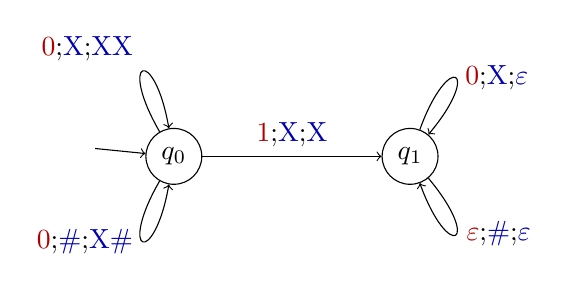
\begin{tikzpicture}
 
    \node[circle,draw] (q0) at (-1.5,0) {$q_0$};
    \node[circle,draw] (q1) at (1.5,0) {$q_1$};
    
    \draw[->] (-2.5,0.1) to  (q0) ;
    
    \draw[->] (q0) edge node[auto] {\el{1}{X}{X}} (q1) ;
    
    \draw[->,in=100, out=120, looseness=22, pos=0.50] (q0) edge node[auto] {\el{0}{X}{XX}} (q0) ;
    \draw[->,in=260, out=240, looseness=22, pos=0.50] (q0) edge node[left] {\el{0}{\#}{X\#}} (q0) ;
    
    \draw[->,in=50, out=70, looseness=22, pos=0.50] (q1) edge node[right] {\el{0}{X}{$\varepsilon$}} (q1) ;
    \draw[->,in=-70, out=-50, looseness=22, pos=0.45] (q1) edge node[right] {\el{$\varepsilon$}{\#}{$\varepsilon$}} (q1) ;
    \end{tikzpicture}
    \end{center}
    
    $010$ wird akzeptiert, weil
        $(q_0, 010, \#)\ConfRel (q_0, 10, X\#)\ConfRel (q_1, 0, X\#)\ConfRel (q_1, \Eps, \#)\ConfRel (q_1, \Eps, \Eps)$.
    
    \begin{center}
    \vspace*{-1.5\baselineskip}
    \begin{minipage}[t]{55mm}
    \begin{align*}
    P_S = \{ 
    & S \to [q_0, \#, q_0]\\
    & S \to [q_0, \#, q_1] 
    \}\\
    \\
    % \end{align*}
    % \begin{align*}
    P_0 = \{ 
    & [q_1, X, q_1] \to 0\\
    & [q_1, \#, q_1] \to \Eps
    \}\\
    \\
    % \end{align*}
    % \begin{align*}
    P_1 = \{ 
    & [q_0, X, q_0] \to 1[q_1, X, q_0]\\
    & [q_0, X, q_1] \to 1[q_1, X, q_1]
    \}
    \end{align*}
    \end{minipage}
    \begin{minipage}[t]{70mm}
    \begin{align*}
    P_2 = \{ 
    & [q_0, \#,q_0] \to 0[q_0, X, q_0] [q_0, \#, q_0]\\
    & [q_0, \#,q_0] \to 0[q_0, X, q_1] [q_1, \#, q_0]\\
    & [q_0, \#,q_1] \to 0[q_0, X, q_0] [q_0, \#, q_1]\\
    & [q_0, \#,q_1] \to 0[q_0, X, q_1] [q_1, \#, q_1]\\
    % 
    & [q_0, X,q_0] \to 0[q_0, X, q_0] [q_0, X, q_0]\\
    & [q_0, X,q_0] \to 0[q_0, X, q_1] [q_1, X, q_0]\\
    & [q_0, X,q_1] \to 0[q_0, X, q_0] [q_0, X, q_1]\\
    & [q_0, X,q_1] \to 0[q_0, X, q_1] [q_1, X, q_1]
    \}
    \end{align*}
    \end{minipage}
    \end{center}
    
    Ableitungsbaum für $010$:
    
    \begin{center}
    \vspace*{-\baselineskip}
    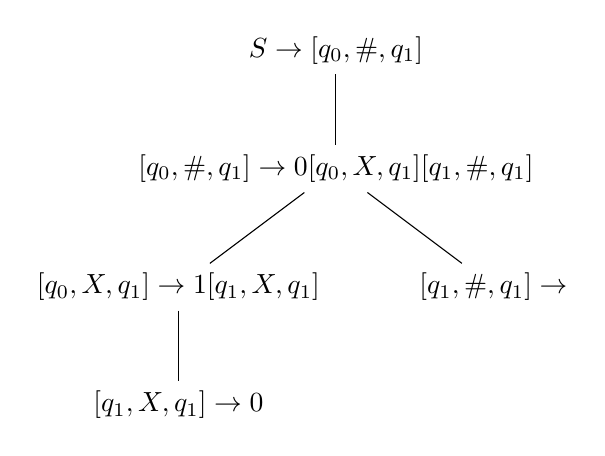
\begin{tikzpicture}
 
    \node[] (root) at (0,0) {$S \to [q_0, \#, q_1]$};
    
    \node[] (m) at (0, -1.5) {$[q_0, \#,q_1] \to 0[q_0, X, q_1] [q_1, \#, q_1]$};
    
    \node[] (ml) at (-2, -3) {$[q_0, X, q_1] \to 1[q_1, X, q_1]$};
    \node[] (mr) at (2, -3) {$[q_1, \#, q_1] \to \Eps$};
    
    \node[] (mlm) at (-2, -4.5) {$[q_1, X, q_1] \to 0$};
    
    
    
    \draw[] (root) to (m) ;
    \draw[] (m) to (ml) ;
    \draw[] (m) to (mr) ;
    \draw[] (ml) to (mlm) ;
    
    \end{tikzpicture}
    \end{center}
    
    Offensichtlich folgt aus dieser Eigenschaft $L(\mathcal{G}) = L(\mathcal{K})$, da wir vom Startsymbol $S$ genau die Nichtterminalsymbole der Form
    $[\qinit, \Zinit, q']$ ableiten können und der \ac{NPDA} genau die Wörter $w$ akzeptiert, für die  $(\qinit, w, \Zinit)$ in eine akzeptierende Konfiguration überführt werden kann.
    
    Es bleibt zu zeigen, dass die Eigenschaft \eqref{eq:npdaToCfgProp} gilt.
    Für den Fall $n=1$ folgt die Eigenschaft direkt aus den $P_0$-Regeln (und der Tatsache, dass keine der anderen Regeln ein einzelnes Symbol oder $\Eps$ ableiten kann).
    
    \begin{itemize}
     \item Beweisrichtung "`$\Rightarrow$"'
     Wir zeigen diese Richtung via vollständige Induktion über die Anzahl der Ableitungsschritte.
     \begin{description}
      \item[I.A.] $n=1$: Folgt wie oben erwähnt aus den $P_0$-Regeln.
      \item[I.S.] $n\rightsquigarrow n+1$:
      Sei $[q,Z,q']\vdash\alpha\stackrel{n}{\vdash} w$ eine Ableitung für $w$. Für den ersten Ableitungsschritt kommen zwei Fälle in Frage:
      \begin{itemize}
      \item Fall 1: $\alpha$ hat die Form $x[q'', Z', q']$ ($[q,Z,q']\rightarrow\alpha \in P_1$).
      
	  Es folgt $w = xw'$ für ein $w'$ mit $[q'', Z', q']\stackrel{n}{\vdash} w'$.
	  
	  Nach I.V.\ gilt nun, dass $(q'', w', Z') \ConfRel^n (q',\Eps,\Eps)$.
	  
	  Nach Konstruktion gilt $\delta(q, x, Z) \ni (q'', Z'), q'' \in Q, x \in \Sigma \cup \{\Eps\}$ und somit
	  $(q, w, Z) \ConfRel (q'', w', Z') \ConfRel^n (q',\Eps,\Eps)$.
      \item Fall 2: $\alpha$ hat die Form $x[q_1,Z_1,q_2][q_2, Z_2, q']$ ($[q,Z,q']\rightarrow\alpha \in P_2$).
      
      Es gibt also einen Ableitungsbaum $\mathcal{T} = \pi(\mathcal{T}_1,\mathcal{T}_2)$, mit $\mathcal{T}_1 \in \operatorname{Abl}([q_1, Z_1, q_2])$ und $\mathcal{T}_2 \in \operatorname{Abl}([q_2, Z_2, q'])$, sodass $w = xY(\mathcal{T}_1)Y(\mathcal{T}_2)$.
      
      Es gilt also $[q_1, Z_1, q_2]\stackrel{k_1}{\vdash} Y(\mathcal{T}_1)$ und 
      $[q_2, Z_2, q']\stackrel{k_2}{\vdash} Y(\mathcal{T}_2)$ für $k_1,k_2\in\N$, sodass $k_1+k_2=n$.
      
          Per I.V.\ folgt
          \begin{displaymath}
            (q_1, Y(\mathcal{T}_1), Z_1) \ConfRel^{k_1} (q_2, \Eps, \Eps).
          \end{displaymath}
          Mit \autoref{lem:4.mehrKeller} folgt auch
          \begin{displaymath}
            (q_1, Y(\mathcal{T}_1)Y(\mathcal{T}_2), Z_1Z_2) \ConfRel^{k_1} (q_2, Y(\mathcal{T}_2), Z_2).
          \end{displaymath}
          

      Auch hier können wir wieder I.V.\ anwenden und erhalten:
          \begin{displaymath}
            (q_2, Y(\mathcal{T}_2), Z_2) \ConfRel^{k_2} (q', \Eps, \Eps)
          \end{displaymath}
          
                    Somit gilt:
          \begin{displaymath}
            (q, \underbrace{xY(\mathcal{T}_1)Y(\mathcal{T}_2)}_{w}, Z) \ConfRel (q_1, Y(\mathcal{T}_1)Y(\mathcal{T}_2), Z_1Z_2) \ConfRel^{k_1} (q_2, Y(\mathcal{T}_2), Z_2) \ConfRel^{k_2} (q', \Eps, \Eps)
          \end{displaymath}
      \end{itemize}
      
     \end{description}

    \end{itemize}
    
    \item Beweisrichtung "`$\Leftarrow$"'
    \datenote{13.12.2017}
     Wir zeigen diese Richtung via vollständige Induktion über die Anzahl der Berechnungsschritte des \ac{NPDA}.
     \begin{description}
      \item[I.A.] $n=1$: Folgt wie oben erwähnt aus den $P_0$-Regeln.
      \item[I.S.] $n\rightsquigarrow n+1$:
      
      Sei $(q,w,Z) \ConfRel^{n+1} (q',\Eps,\Eps)$ eine Berechnung für $w$. Da wir annehmen, 
      dass der \ac{NPDA} in einem Schritt höchstens zwei Symbole auf den Stack legen darf, kommen für den ersten Berechnungsschritt nur zwei Fälle in Frage:
      \begin{itemize}
      \item Fall 1: $(q,w,Z)\ConfRel (q'', w',Z')$ mit $w=xw'$ für $x\in\Sigma\cup\{\Eps\}$
      
      Aus $(q'', w',Z')\ConfRel^n (q',\Eps,\Eps)$ folgern wir mit I.V.\
      $[q'', Z',q']\vdash^n w'$.
      Nach Konstruktion können wir $[q,Z,q']\vdash x [q'', Z',q']$ ableiten.

      
      \item Fall 2: $(q,w,Z)\ConfRel (q_1, w',Z_1Z_2)$ mit $w=xw'$ für $x\in\Sigma\cup\{\Eps\}$

            Aus $(q_1, w',Z_1Z_2)\ConfRel^n (q',\Eps,\Eps)$ folgern wir:
      $\exists k_1,k_2\in\N, \; q_2\in Q, \; w_1,w_2\in \Sigma^*$, sodass gilt:
      \begin{enumerate}
      \item $k_1+k_2=n$
      \item $w'=w_1w_2$
      \item $(q_1, w',Z_1Z_2)\ConfRel^{k_1} (q_2, w_2,Z_2)$
      \item $(q_2, w_2,Z_2)\ConfRel^{k_2} (q',\Eps,\Eps)$
      \end{enumerate}
      Wir wählen $k_1$ als die kleinste Zahl, welche die obigen Eigenschaften erfüllt.
      Damit wissen wir, dass wir $Z_2$ noch nie vom Keller genommen haben.
      
      Aus 3.\ folgern wir $(q_1, w_1,Z_1)\ConfRel^{k_1} (q_2, \Eps,\Eps)$ und mit I.V.\
      $[q_1, Z_1, q_2] \vdash^{k_1} w_1$.
      
      Aus 4.\ folgern wir mit I.V.\ $[q_2, Z_2, q'] \vdash^{k_2} w_2$.
      
      Es gibt also einen Ableitungsbaum $\mathcal{T} = \pi(\mathcal{T}_1,\mathcal{T}_2)$, mit $\mathcal{T}_1 \in \operatorname{Abl}([q_1, Z_1, q_2])$ und $\mathcal{T}_2 \in \operatorname{Abl}([q_2, Z_2, q'])$, sodass $w = xY(\mathcal{T}_1)Y(\mathcal{T}_2)$.
      
      Somit gibt es auch eine Ableitung
      \begin{equation*}
      [q, Z, q'] \vdash x[q_1,Z_1,q_2][q_2, Z_2, q'] \vdash^{k_1+k_2} xw_1w_2. \qedhere
      \end{equation*}
      \end{itemize}
     \end{description}
\end{proof}

\begin{Satz}
Die Menge der von Kellerautomaten akzeptierten Sprachen und die Menge der kontextfreien Sprachen sind identisch.
\end{Satz}
\begin{proof}
Folgt direkt aus \autoref{lem:4.cfgToNpda} und \autoref{lem:4.npdaToCfg}.
\end{proof}

\begin{Bemerkung}
Zu jedem \ac{NPDA} gibt es einen äquivalenten \ac{NPDA}, der nur einen Zustand hat.
(Folgt aus \autoref{lem:4.npdaToCfg} und der Konstruktion aus dem Beweis von \autoref{lem:4.cfgToNpda}.)
\end{Bemerkung}



\section{Kontextfreie Sprachen -- Teil 2}

\subsection{Das Pumping Lemma für kontextfreie Sprachen}
\begin{Satz}[Pumping Lemma für \acs*{CFL}]
\label{satz:PL für CFL}
%\rlnote{Satz \# 4.2?}
	Sei $L$ eine kontextfreie Sprache. Dann gilt:
	        \begin{alignat*}{2}
                &\exists n\in\N,\ n>0:\quad \forall z\in L,\ |z|\geq n:\\
                &\exists u,v,w,x,y\in\Sigma^* :\\
                &z = uvwxy,\ |vwx| \leq n,\ |vx| \geq 1\\
                \text{und }& \forall i\in\N: uv^iwx^iy\in L
        \qedhere
        \end{alignat*}
\end{Satz}
\begin{lemma}\label{lemma:Binärbaum}
 In jedem Binärbaum (Baum, bei dem jeder innere Knoten zwei Nachfolger hat) mit $\geq 2^k$ Blättern gibt es mindestens einen Pfad der Länge $\geq k$ von einem Blatt zur Wurzel.
\end{lemma}
(ohne Beweis)

\begin{proof}[von \autoref{satz:PL für CFL}]
	Sei $\mathcal{G}= (\Sigma,N,P,S)$ in \ac{CNF} mit
    $L(\mathcal{G}) = L$. Wähle $n=2^{|N|}$.
    
     Betrachte den Ableitungsbaum $\mathcal{T} \in \operatorname{Abl}(S)$ für ein Wort $z$ mit $|z|\geq n$. 
%     \footnote{Intuition: Da $\mathcal{G}$ in \ac{CNF}, ist Ableitungsbaum $\mathcal{T}$ ein Binärbaum. 
%         Mit $|N|$ 
%     verschiedenen Nichtterminalsymbolen kann man 
%     also maximal Wörter der Länge $2^{|N|}$ ableiten, wenn man keine Ableitung doppelt nutzen möchte. 
%     Leitet man ein längeres Wort ab, so muss man mind. eine Ableitung doppelt nutzen.
%      Dann kann man sie aber auch gleich $i$-fach nutzen ($v^i$ und $x^i$), und ist immernoch in der Sprache.}
  $\mathcal{T}$ ist ein Binärbaum mit $|z|\geq n = 2^{|N|}$ Blättern.
  In einem solchen Binärbaum existiert nach \autoref{lemma:Binärbaum} ein Pfad $\zeta$ der Länge $\geq |N|$.
	Auf $\zeta$ liegen $\geq |N|+1$ Nichtterminalsymbole.
	Es muss also mindestens ein Nichtterminalsymbol $A$ mehrmals vorkommen.
	
  Folge $\zeta$ vom Blatt in Richtung Wurzel, bis sich ein Nichtterminalsymbol $A$ das erste Mal wiederholt. Das geschieht nach $\le |N|$ Schritten.
  Teile $z = uvwxy$ wie in \autoref{zerlegung} skizziert. Es gilt:
      \begin{itemize}
      \item $|vx|\geq 1$, da $\zeta$ entweder durch $B$ oder durch $C$ läuft.
        Angenommen, $\zeta$ verläuft durch $B$.
        Somit muss $C \stackrel{*}{\vdash} x$ gelten. In \ac{CNF} ist $C \stackrel{*}{\vdash} \Eps$ nicht möglich und somit ist $|x| \ge 1$.
        Der Fall, dass $\zeta$ durch $C$ verläuft, ist analog.
      \item $|vwx| \le 2^{|N|} = n$, da das obere $A$ höchstens $|N|$ Schritte von der Blattebene entfernt und $\mathcal{T}$ ein Binärbaum ist.
      \item Für die Aussage $\forall i\in\N: uv^iwx^iy\in L$ unterscheiden wir drei Fälle:
      \begin{itemize}
				\item $i=0$: Aus dem "`unteren"' $A$ haben wir $w$ abgeleitet,
				aus dem oberen $A$ haben wir $vwx$ abgeleitet.
				Wir könnten also auch aus dem oberen $A$ direkt $w$ ableiten und erhalten $S\vdash^* uwy$.
				(Siehe \autoref{uv0wx0y}).
				\item $i=1$: Gilt trivialerweise, da $uv^1wx^1y=z$.
				\item $i\geq 1$: Aus dem "`oberen"' $A$ haben wir $vAx$ abgeleitet,
				aus dem unteren $A$ haben wir $w$ abgeleitet.
				Wir könnten also auch aus dem unteren $A$ nochmal $vAx$ ableiten.
				Wenn wir dies oft genug wiederholen, können wir jedes $uv^iwx^iy$ mit $i\geq 2$ erzeugen
				(siehe auch \autoref{uviwxiy}).
				
      \end{itemize}

      \end{itemize}
		\begin{figure}[H]\centering
		\begin{subfigure}[b]{.35\linewidth}\centering
					\begin{tikzpicture}[>=stealth,
				widebox/.style={draw, minimum width=.75cm, minimum height=.35cm, inner sep=0pt}
				,dot/.style={inner sep=0pt,outer sep=0pt,label={center:\scalebox{.75}{\textbullet}}}
				]
				
				\node[dot,label={above right:$S$}] (v1) at (0,-1) {};
				\node[dot] (v2) at (-0.25,-1.6) {};
				\node[dot,] (v3) at (0,-2) {};
				\node[dot] (v4) at (-0.5,-2.5) {};
				\node[dot,label={above right:$A$}] (v5) at (0,-3) {};
				\node[widebox] (v6) at (-1.5,-3.5) {$u$};
				\node[widebox] (v7) at (-.75,-3.5) {$v$};
				\node[widebox] (v8) at (0,-3.5) {$w$};
				\node[widebox] (v9) at (.75,-3.5) {$x$};
				\node[widebox] (v10) at (1.5,-3.5) {$y$};
				
				\draw  (v1) edge (v2);
				\draw  (v2) edge (v3);
				\draw  (v3) edge (v4);
				\draw  (v4) edge (v7.north west);
				\draw  (v4) edge (v5);
				\draw  (v3) edge (v10.north west);
				\draw  (v5) edge (v8.north west);
				\draw  (v5) edge (v8.north east);
				\draw  (v1) edge (v6.north west);
				\draw  (v1) edge (v10.north east);
				\node[align=left,inner sep=2pt] at (1.7,-1.4) {$A\rightarrow BC$} edge[->,shorten >=.1cm] (v3);
				\node[inner sep=0pt] at (2.75,-3.0) {$A\rightarrow a$} edge[->] (v10);
				\node (v11) at (0,-4) {$z$};
				\draw[semithick]
				let \p1 = (v6.west), \p2 = (v11), \p3 = (v10.east) in 
				 (\x1,\y2) edge[{Bar[]<}-] (v11) (v11) edge[-{>Bar[]}] (\x3,\y2);
			\end{tikzpicture}
					\caption{Zerlegung $z = uvwxy$}\label{zerlegung}
		\end{subfigure}
		\begin{subfigure}[b]{.28\linewidth}\centering
			\begin{tikzpicture}[node distance=.5cm, on grid,
					every node/.style={
						execute at begin node=$,
						execute at end node=$
					},
					widebox/.style={draw, minimum width=.75cm, minimum height=.35cm, inner sep=0pt}
				]
				\node (S) {S};
				\node[inner sep=2pt] (A) [below=of S.south, xshift=.2cm] {A};
				\coordinate (Ap) at (A.south west);
				\node[widebox] (w) [below=of Ap] {w};
				\node[widebox] (u) at ($(Ap)!2!(w.north west)+.5*(-.75,-.3)$) {u};
				\node[widebox] (y) at ($(Ap)!2!(w.north east)+.5*(.75,-.3)$) {y};
				
				\draw (S.south) edge (u.north west) edge (y.north east)
					(Ap) edge (u.north east) edge (y.north west) edge (w.north)
					($(S.south) - (.25,.6)$) edge (S.south) edge (Ap)
				;
			\end{tikzpicture}
			\caption{$uwy\in L$}\label{uv0wx0y}
		\end{subfigure}
		\begin{subfigure}[b]{.29\linewidth}\centering
			\begin{tikzpicture}[node distance=.75cm, on grid,
					every node/.style={
						execute at begin node=$,
						execute at end node=$
					}
				]
				\node (0) {S};
				\node (A1) [below=of 0] {A};
				\node (A2) [below=of A1] {A};
				\node (A3) [below=of A2] {A};
				
				\newlength\Offset \setlength\Offset{.75cm}
				\coordinate(p1) at ($(A2.south) - (0,\Offset)$);
				%
				\coordinate (A2l) at ($(p1) - (\Offset,0)$);
				\coordinate (A1l) at ($(A2l) - (\Offset,0)$);
				\coordinate (0l) at ($(A1l) - (\Offset,0)$);
				%
				\coordinate (A2r) at ($(p1) + (\Offset,0)$);
				\coordinate (A1r) at ($(A2r) + (\Offset,0)$);
				\coordinate (0r) at ($(A1r) + (\Offset,0)$) ;
				
				\coordinate (A3l) at ($(A3.south) - (\Offset,\Offset)$);
				\coordinate (A2l2) at ($(A3l) - (\Offset,0)$);
				%
				\coordinate (A3r) at ($(A3.south) + (\Offset,-\Offset)$);
				\coordinate (A2r2) at ($(A3r) + (\Offset,0)$);
				
				\node (dots) [below=\Offset of A3] {\vdots};
				
				\node (A4) [below=\Offset of dots] {A};
				\coordinate (A4l) at ($(A3l) - (0,2*\Offset)$);
				\coordinate (A4r) at ($(A3r) - (0,2*\Offset)$);
				
				\draw (0.south) edge (0l.center) edge (0r.center)
					(A1.south) edge (A1l.center) edge (A1r.center)
					(A2.south) edge (A2l2.center) edge (A2r2.center)
					(A3.south) edge (A3l.center) edge (A3r.center)
					(A4.south) edge (A4l.center) edge (A4r.center)
				;
				\draw (0l.center) edge node[below] {u} (A1l.center)
					(A1l.center)  edge node[below] {v} (A2l.center)
					(A2r.center)  edge node[below] {x} (A1r.center)
					(A1r.center)  edge node[below] {y} (0r.center)
					(A2l2.center) edge node[below] {v} (A3l.center)
					(A3r.center)  edge node[below] {x} (A2r2.center)
					(A4l.center)  edge node[below] {w} (A4r.center)
				;
			\end{tikzpicture}
			\caption{$uv^iwx^iy\in L$}\label{uviwxiy}
		\end{subfigure}
% 		\begin{subfigure}[b]{.33\linewidth}\centering
% 			\begin{tikzpicture}[>=stealth,
% 				widebox/.style={draw, minimum width=.75cm, minimum height=.35cm, inner sep=0pt}
% 				,dot/.style={inner sep=0pt,outer sep=0pt,label={center:\scalebox{.75}{\textbullet}}}
% 				]
% 				
% 				\node[dot,label={above right:$S$}] (v1) at (0,-1) {};
% 				\node[dot] (v2) at (-0.25,-1.6) {};
% 				\node[dot,label={above right:$A$}] (v3) at (0,-2) {};
% 				\node[dot] (v4) at (-0.5,-2.5) {};
% 				\node[dot,label={above right:$A$}] (v5) at (0,-3) {};
% 				\node[widebox] (v6) at (-1.5,-3.5) {$u$};
% 				\node[widebox] (v7) at (-.75,-3.5) {$v$};
% 				\node[widebox] (v8) at (0,-3.5) {$w$};
% 				\node[widebox] (v9) at (.75,-3.5) {$x$};
% 				\node[widebox] (v10) at (1.5,-3.5) {$y$};
% 				
% 				\draw  (v1) edge (v2);
% 				\draw  (v2) edge (v3);
% 				\draw  (v3) edge (v4);
% 				\draw  (v4) edge (v7.north west);
% 				\draw  (v4) edge (v5);
% 				\draw  (v3) edge (v10.north west);
% 				\draw  (v5) edge (v8.north west);
% 				\draw  (v5) edge (v8.north east);
% 				\draw  (v1) edge (v6.north west);
% 				\draw  (v1) edge (v10.north east);
% 				\node[align=left, text height=3em,inner sep=2pt] at (2.1,-1.5) {$A\rightarrow BC$\small{ist Binärbaum}} edge[->,shorten >=.1cm] (v3);
% 				\node[inner sep=0pt] at (2.75,-3.5) {$A\rightarrow a$} edge[->] (v10);
% 				\node (v11) at (0,-4) {$z$};
% 				\draw[semithick]
% 				let \p1 = (v6.west), \p2 = (v11), \p3 = (v10.east) in 
% 				 (\x1,\y2) edge[{Bar[]<}-] (v11) (v11) edge[-{>Bar[]}] (\x3,\y2);
% 			\end{tikzpicture}
% 			\caption{$\exists$ Pfad mit Länge $\geq k$}
% 		\end{subfigure}
		\caption{Erklärung zu \autoref{satz:PL für CFL}}
	\end{figure}\vspace{-2em}\qedhere
\end{proof}

\begin{lemma}\label{bsp:5.planbncn}
\datenote{15.12.2017}
Die Sprache $L=\{a^nb^nc^n \mid n\geq 1\}$ ist nicht kontextfrei.
\end{lemma}
\begin{proof}
  Wir nehmen an, $L$ wäre kontextfrei.
	Sei $n$ die Konstante aus dem \ac{PL}.
	Wir betrachten $z=a^nb^nc^n$. Es gilt also $|z| = 3n \ge n$.
  Dann gibt es eine Zerlegung $z = uvwxy$ mit $|vx| \ge 1$ und $|vwx| \le n$.
  Wir zeigen nun, dass $\forall i\in\N: uv^iwx^iy\in L$ nicht gilt (und folgern, dass unsere Annahme falsch war).

  Durch $|vwx| \le n$ ergeben sich für $vwx$ folgende Möglichkeiten:
  \begin{itemize}
  \item $vwx = a^j$: 
    Für $i=0$ ist $v^0wx^0=w$ mit $|w| < j$.
    Die Anzahl der $a$ stimmt also nicht mehr mit der Anzahl der $b$ überein.
  \item $vwx = a^kb^j$:
    \begin{itemize}
    \item Falls $v = a^{k'}$, $x = b^{j'}$: Für $i=0$ stimmt die Anzahl der $a$ oder die Anzahl der $b$ nicht mehr mit der Anzahl der $c$ überein.
    \item Falls $v$ ein Gemisch aus $a$ und $b$ enthält:
      Für $i\ge 2$ würde eine Folge $a^n$ durch eine $b$-Folge unterbrochen.
    \item Falls $x$ ein Gemisch aus $a$ und $b$ enthält:
      Für $i \ge2$ würde eine Folge $a^n$ durch eine $b$-Folge unterbrochen.
    \end{itemize}
  \item $vwx = b^j$: analog zu Fall $a^j$
  \item $vwx = b^kc^j$: analog zu Fall $a^kb^j$
  \item $vwx = c^j$: analog zu Fall $a^j$
  \end{itemize}
  In jeder der Möglichkeiten lässt sich also durch "`Pumpen"' ein Wort $w \not \in L$ finden.
  Daher kann $L$ nicht kontextfrei sein.
\end{proof}




\begin{lemma} %\rlnote{Lemma \# 4.3?}

  Die Menge der kontextfreien Sprachen ($\mathcal{M}_2$) ist eine echte Teilmenge der Menge der kontextsensitiven Sprachen ($\mathcal{M}_1$).
\end{lemma}
\begin{proof}
Aus \autoref{beob:3.ChomskyHierarchie} wissen wir bereits, dass $\mathcal{M}_2 \subseteq \mathcal{M}_1$ gilt.
Aus \autoref{bsp:3.anbncn} wissen wir, dass $L=\{a^nb^nc^n \mid n\geq 1\}$ von einer kontextsensitiven Grammatik erzeugt wird.
Mit Hilfe von \autoref{bsp:5.planbncn} folgern wir $\mathcal{M}_2 \subsetneq \mathcal{M}_1$.
\end{proof}

% \begin{Bsp} Die Sprache
%   \begin{displaymath}
%     L = \{ww \mid w \in \{a,b\}^*\}
%   \end{displaymath}
%   ist kontextsensitiv aber nicht kontextfrei.
% 
%   Sei $n$ die Konstante aus dem PL
% 
%   Betrachte $z = a^nb^na^nb^n \in L$ mit $|z| = 4n \ge n$.
%   Nach PL ist $z = uvwxy$ mit $|vx| \ge 1$ und $|vwx| \le n$.
% 
%   Es ergeben sich folgende Möglichkeiten:
%   \begin{itemize}
%   \item $vwx = a^j$, $j \le n$.
%     Für $i=0$ ist $vwx=w$ mit $|w| < j$.
%     Anzahl der $a$ stimmt nicht mehr mit $n$ überein.
%   \item $vwx = a^kb^j$, $k+j \le n$.
% 
%     \begin{itemize}
%     \item Falls $v = a^{k'}$, $x = b^{j'}$: Für $i=0$ stimmt die Anzahl der $a$ nicht mehr mit $n$ überein.
%     \item Falls $v$ ein Gemisch aus $a$ und b enthält.
%       Für $i>2$ würde eine Folge $a^n$ durch eine $b$-Folge unterbrochen.
%     \item Falls $x$ ein Gemisch aus $a$ und b enthält.
%       Für $i>2$ würde eine Folge $a^n$ durch eine $b$-Folge unterbrochen.
%     \end{itemize}
%   \item $vwx = b^j$ analog Fall $a^j$
%   \item $vwx = b^ka^j$ analog Fall $a^kb^j$
%   \end{itemize}
% \end{Bsp}


\subsection{Abschlusseigenschaften für kontextfreie Sprachen}
\begin{Satz} % 4.7
  \label{thm:cfl-closed-reg-intersect}
	Die \ac{CFL} ist abgeschlossen unter Vereinigung ($\cup$), Konkatenation ($\cdot$) und dem Sternoperator ($^*$).
\end{Satz}
\begin{proof}
	Für zwei \ac{CFG} $\mathcal{G}_i = (\Sigma, N_i, P_i,S_i), i=1,2$, konstruiere $\mathcal{G} = (\Sigma, N,P,S)$ mit
	\begin{align*}
		\text{"`}\cup\text{"'}: N &= N_1\dotcup N_2\dotcup\{S\}\\
		P &= \{S\->S_1, S\->S_2 \} \cup P_1\cup P_2\\
		\text{"`}\cdot\text{"'}: N &= N_1\dotcup N_2\dotcup\{S\}\\
		P &= \{ S\->S_1S_2 \} \cup P_1\cup P_2\\
		\text{"`}^*\text{"'}: N &= N_1 \dotcup \{S\}\\
		P &= \{ S\->\Eps, S\-> S_1S \} \dotcup P_1
	\qedhere
	\end{align*}
\end{proof}

\begin{Satz}
 	Die \ac{CFL} sind \emph{nicht} unter Schnitt ($\cap$) abgeschlossen.
\end{Satz}
\begin{proof}
 für $n\geq 1$
		\[ \underbrace{\{a^nb^nc^m \mid n,m\geq 1 \}}_{\in \acs{CFL}} \cap \underbrace{\{a^mb^nc^n \mid m,n\geq 1 \}}_{\in \acs{CFL}} = \underbrace{\{a^nb^nc^n\}}_{\notin \acs{CFL}} \]
		Also \ac{CFL} nicht abgeschlossen unter $\cap$.
		(siehe \autoref{bsp:5.planbncn})
\end{proof}


\begin{Satz}
 	Die \ac{CFL} sind \emph{nicht} unter Komplement ($\overline{\!\phantom{i}\cdot\!\phantom{i}}$) abgeschlossen.
\end{Satz}
\begin{proof}
Angenommen, CFL wäre abgeschlossen unter $\overline{\!\phantom{i}\cdot\!\phantom{i}}$.\\
		Falls $L_1,L_2\in \acs*{CFL}$, dann ist $\overline{L}_1,\overline{L}_2\in\acs*{CFL}$ nach Annahme.\\
		$\Rightarrow \overline{L}_1\cup \overline{L}_2\in\acs*{CFL}$ wegen Abschluss unter "`$\cup$"'.\\
		$\Rightarrow \overline{\overline{L}_1\cup \overline{L}_2} = L_1\cap L_2\in\acs*{CFL}$ -- Widerspruch zu Nicht-Abschluss unter "`$\cap$"'. \qedhere
\end{proof}



\subsection{Deterministisch kontextfreie Sprachen}

\begin{Def}
Wir definieren einen \emph{Kellerautomaten mit akzeptierenden Zuständen} als 7-Tupel
\[
	\mathcal{E} = (\Sigma,Q,\Gamma,q^\text{init},\Zinit,\delta,F)
\]
mit den Komponenten $\Sigma,Q,\Gamma,q^\text{init},\Zinit,\delta$ wie für einen gewöhnlichen Kellerautomaten und $F \subseteq Q$ als die Menge der akzeptierenden Zustände.

\smallskip

Weiterhin definieren wir das Akzeptanzverhalten folgendermaßen: \\
Eine Konfiguration $(q, w, \gamma)$ eines Kellerautomaten mit akzeptierenden Zuständen ist \emph{akzeptierend}, falls $q \in F$ und $w = \varepsilon$.
Die von einem Kellerautomaten mit akzeptierenden Zuständen $\mathcal{E}$ \emph{akzeptierte Sprache} ist
\[
	L(\mathcal{E}) = \{w \in \Sigma^* \mid \exists q \in F, \gamma \in \Gamma^*: (q^\text{init}, w, Z^\text{init}) \ConfRel^* (q, \varepsilon, \gamma)\}.
\]
Hierbei ist $\ConfRel$ die Schrittrelation genau wie für gewöhnliche Kellerautomaten.
\end{Def}

\begin{lemma}
Zu jedem (gewöhnlichen) Kellerautomaten gibt es einen Kellerautomaten mit akzeptierenden Zuständen, der die gleiche Sprache akzeptiert.
Gleiches gilt in die andere Richtung.
\end{lemma}
\begin{proof}
Siehe Übungsblatt~7 Aufgabe~5.
\end{proof}




\begin{Def}[name={[DPDA]}]
        Ein \ac{DPDA} ist ein 7-Tupel
        $$\mathcal{D} = (\underbrace{\Sigma,Q,\Gamma,\qinit,\Zinit}_{\text{wie gehabt}},\delta,F)$$
        \vspace{-1em}
        \begin{itemize}
        \item $F\subseteq Q$ akzeptierende Zustände
        \item $\delta: Q\x (\Sigma\cup\{\Eps\})\x \Gamma \-> \mathcal{P}(Q\x \Gamma^*)$ wobei für alle $q\in Q,a\in\Sigma,Z\in\Gamma$ gelten muss, dass
        $|\delta(q,a,Z)| + |\delta(q,\Eps,Z)| \leq 1$
        \item Die Schrittrelation "`$\ConfRel$"' ist definiert wie bei \ac{NPDA}s.
        \item $L(\mathcal{D}) = \{w\in\Sigma^* \mid (\qinit,w,\Zinit) \ConfRel^* (q',\Eps,\gamma) \land q'\in F \}$ \qedhere
        \end{itemize}
\end{Def}

\begin{lemma}[name={[\acs*{DPDA}, der gesamte Eingabe verarbeitet]}]
        \label{lem:DPDA ges. Eingabe}
        Zu jedem \ac{DPDA} $\mathcal{D}$ gibt es einen äquivalenten \ac{DPDA} $\mathcal{D}_e$, der
        jede Eingabe bis zum Ende liest.
\end{lemma}
% \draftnote{23.12.16}
\begin{proof}

  Sei $\mathcal{D} = (\Sigma, Q, \Gamma, \qinit, \Zinit, \delta, F)$. 
  Es gibt zwei Möglichkeiten, warum $\mathcal{D}$ nicht die gesamte Eingabe verarbeitet:
  Die Transitionsrelation ist nicht total 
%   \footnote{
%   d.h. es gibt Konfigurationen mit nicht-leerem Keller
%   so dass $a \not \Rightarrow^* b$} 
  oder der Automat bleibt bei
  leerem Keller stecken.

  Abhilfe: Führe einen Senkzustand ein, auf dem $\mathcal{D}_S$ weiterrechnet, wenn $\mathcal{D}$ nicht mehr weiterrechnen kann. 
  Definiere dazu $\mathcal{D}_S = (\Sigma, Q_S, \Gamma_S, \qinit_S, \Zinit_S, \delta_S, F_S)$ mit
  \begin{align*}
  Q_S &= Q \cup \{\qinit_S, q_s\} \text{ mit neuen Zuständen: $\qinit_S$ neuer Startzustand und $q_s$ Senkzustand} \\
  F_S &= F \\
  \Gamma_S &= \Gamma \cup \{\Zinit_S\} \text{ neues Kellerbodensymbol}
  \end{align*}
  und Transitionsfunktion $\delta_S$ gegeben durch
  \[\delta_S (\qinit_S, \varepsilon, \Zinit_S) = \{ (\qinit, \Zinit\Zinit_S) \} \]
  \begin{itemize}
  \item Transitionsfunktion totalisieren: Für alle $q\in Q$, $Z \in \Gamma$
    \begin{align*}
      \delta_S (q, \varepsilon, Z) &=
      \begin{cases}
        \delta (q, \varepsilon, Z) & \text{falls
        }\delta (q, \Eps, Z)\ne\emptyset\vee\exists a\in\Sigma, \delta (q, a, Z)\ne \emptyset \\
        \{ (q_s, Z) \} & \text{sonst}
      \end{cases} \\
      \delta_S (q, a, Z) &=
      \begin{cases}
        \delta (q, a, Z) & \text{falls }\delta (q, \Eps, Z)\ne\emptyset\vee\delta (q,
        a, Z) \ne \emptyset \\
        \{ (q_s, Z) \} & \text{sonst}
      \end{cases}
    \end{align*}
    Intuition: Wenn $\delta(q, a, Z) = \emptyset$ und es keinen $\epsilon$-Übergang gibt, kann das Wort von $\mathcal{D}$ nicht weiter abgearbeitet werden. $\mathcal{D}_S$ geht nun in Senkzustand $q_s$ und arbeitet dort weiter. Analog für $\delta(q, \epsilon, Z)$.
  \item Kellerunterlauf vermeiden: $\mathcal{D}$ hat $\Zinit$ abgeräumt, so dass $\Zinit_S$
    sichtbar geworden ist. Füge eine $\epsilon$-Transition in
     Senkzustand $q_s$ hinzu, indem man für alle $q\in Q$ definiert:
    \[\delta_S (q, \varepsilon, \Zinit_S) = \{ (q_s, \Zinit_S) \} \]
  In $q_s$ kann $\mathcal{D}_S$ nun das Restwort für alle $a\in\Sigma$, $Z\in \Gamma_S$ abarbeiten:
    \[\delta_S (q_s, a, Z) = \{ (q_s, Z) \}\]
    Bemerkung: $q_s \not \in F_S$, da ein Kellerunterlauf
    das Akzeptieren des eingelesen Worts ausschließt.
  \end{itemize}

  Es verbleibt zu zeigen:
  \begin{itemize}
   \item $\forall w\in \Sigma^*$ $\exists q\in Q_S$,
  $\gamma\in\Gamma_S^*: (\qinit_S, w, \Zinit_S) \ConfRel^* (q,
  \varepsilon, \gamma)$.
  
  (Induktion über die Länge von $w$)
  \item $L (\mathcal{D}) = L (\mathcal{D}_S)$.
  \qedhere
  \end{itemize}
\end{proof}

\begin{Satz}[name={[Abgeschlossenheit der deterministischen \acs*{CFL}]}]
        Die deterministischen \ac{CFL} sind unter Komplement abgeschlossen.
\end{Satz}
\begin{proof}
  Sei $L$ deterministisch kontextfrei. 
  Nach \autoref{lem:DPDA ges. Eingabe} gibt es einen \ac{DPDA} $\mathcal{D}$ mit $L(\mathcal{D})=L$, der die komplette Eingabe liest.

  Konstruiere einen \ac{DPDA} $\mathcal{D}_K$, sodass $ L(\mathcal{D}_K) = \overline{L}$. 
  Definiere dazu $Q_K= Q \times \{0,1,2\}$. Bedeutung des zusätzlichen "`Flags"' in $\{0,1,2\}$:
  \begin{itemize}
  \item $0$: seit dem Lesen des letzten Symbols $a \in \Sigma$ wurde kein akzeptierender Zustand durchlaufen
  \item $1$: seit dem Lesen des letzten Symbols $a \in \Sigma$ wurde mindestens ein
    akzeptierender Zustand durchlaufen 
  \item $2$: markiert einen akzeptierenden Zustand in $\mathcal{D}_K$
  \end{itemize}
        
  $F_K=F\x \{2\}$

  Definiere Hilfsfunktion $\mathit{acc}:Q\to \{0,1\}$ durch 
  \begin{displaymath}
    \mathit{acc} (q) =
    \begin{cases}
      0 & q\notin F \\ 1 & q \in F
    \end{cases}
  \end{displaymath}
  \begin{align*}
    \qinit_K &= (\qinit,\mathit{acc} (\qinit))
  \end{align*}
  Wir definieren $\delta'$ für alle $q \in Q$, $Z\in\Gamma$ folgendermaßen.
  
  Falls $\delta(q,\Eps,Z) = \{(q',\gamma)\}$, dann
  \begin{align*}
    \delta'((q,0),\Eps,Z) &= ((q',\mathit{acc} (q')),\gamma)
    \\
    \delta'((q,1),\Eps,Z) &= ((q',1),\gamma)
  \end{align*}
  Falls $\delta(q,a,Z) = \{(q',\gamma)\}$, dann
  \begin{align*}
    \delta'((q,0), \Eps, Z) &= \{ ((q,2), Z) \} \\
    \delta'((q,2), a, Z) &=((q',\mathit{acc} (q')), \gamma)
    \\
    \delta'((q,1), a, Z) &=
    ((q',\mathit{acc} (q')), \gamma)
    \qedhere    %TODO Intuition?
  \end{align*}
\end{proof}

\begin{Satz}
Die deterministisch kontextfreien Sprachen sind eine echte Teilmenge der kontextfreien Sprachen.
\end{Satz}

\begin{proof}
 Offensichtlich gibt es eine Teilmengenbeziehung, denn die von nichtdeterministischen Kellerautomaten mit akzeptierendem Zustand akzeptierten Sprachen sind gerade die kontextfreien Sprachen und jeder deterministische Kellerautomat ist ein spezieller nichtdeterminischer Kellerautomaten mit akzeptierenden Zuständen.
 Die deterministisch kontextfreien Sprachen sind unter Komplement abgeschlossen, die kontextfreien Sprachen sind es nicht.
 Die beiden Mengen von Sprachen können also nicht gleich sein.
\end{proof}



\hide{

\begin{Satz}
    Die deterministischen \ac{CFL} sind \textbf{nicht} unter Vereinigung und Durchschnitt abgeschlossen.
\end{Satz}
\begin{proof}
    Betrachte
    \begin{align*}
        L_1 &= \{ a^nb^nc^m \mid n, m \ge 1 \} \\
        L_2 &= \{ a^mb^nc^n \mid n, m \ge 1 \}
    \end{align*}
    Sowohl $L_1$ als auch $L_2$ sind DCFL, aber $L_1 \cap L_2 = \{ a^nb^nc^n \mid n \ge 1\}$ ist nicht kontextfrei.
    
    DCFL ist nicht abgeschlossen unter Vereinigung. Angenommen doch: Seien $U, V$ DCFL. Dann sind auch $\overline{U}$ und $\overline{V}$ DCFL. Bei Abschluss unter Vereinigung wäre $\overline{U} \cup \overline{V}$ eine DCFL und somit auch $\overline{\overline{U} \cup \overline{V}} = U \cap V$, ein Widerspruch gegen den ersten Teil.
\end{proof}
\begin{Satz}
    DCFL ist abgeschlossen unter Schnitt mit REG.
\end{Satz}
\begin{proof}
    Sei $L$ DCFL und $R$ regulär.
    Konstruiere das Produkt aus einem DPDA für $L$ und einem DFA für $R$.
    Offenbar ist das Ergebnis ein DPDA, der $L\cap R$ akzeptiert. \footnote{
    Intution des Beweis: Konstruiere Produktautomaten, der akzeptiert gdw. der DFA und NDPA akzeptieren. Idee: Definiere Tupel $(q_1, q_2)$, DPDA arbeitet auf $q_1$, DFA arbeitet auf $q_2$. Beispielsweise werden $\epsilon$-Übergänge des DPDA nur auf der "`DPDA-Seite"' d.h. auf $q_1$ abgearbeitet, ohne Beeinflussung von $q_2$.
    }

    $L = L (M_1)$ mit $M_1 = (Q_1, \Sigma, \Gamma, q_{01}, \Zinit,
    \delta_1, F_1)$ \ac{DPDA}

    $R = L (M_2)$ mit $M_2 = (Q_2, \Sigma, q_{02}, \delta_2, F_2)$
    \ac{DFA}

    Konstruiere $M'= (Q, \Sigma, \Gamma, \qinit, \Zinit, \delta, F)$ mit
    \begin{itemize}
    \item $Q = Q_1 \times Q_2$
    \item $\qinit = (q_{01}, q_{02})$
    \item $F = F_1  \times F_2$
    \item Falls $\delta_1 (q_1, \varepsilon, Z) = \{(q_1', \gamma)\}$, dann gilt für alle $q_2\in Q_2$: 
      \[ \delta ((q_1, q_2), \varepsilon, Z)
      = \{((q_1', q_2), \gamma)\} \text{.     (Ansonsten leer)} \]
    \item Falls $\delta_1 (q_1, a, Z) = \{(q_1', \gamma)\}$, dann gilt für alle $q_2\in Q_2$: 
      \[ \delta ((q_1, q_2), a, Z) =
      \{((q_1', \delta_2 (q_2, a)), \gamma)\} \text{   (Ansonsten leer)} \]
    \end{itemize}
    Zu zeigen ist noch $L (M') = L (M_1) \cap L (M_2)$.
\end{proof}
\begin{Satz}
    Sei $L$ DCFL und $R$ regulär.
    Es ist entscheidbar, ob $R=L$, $R\subseteq L$ und $L=\Sigma^*$.
\end{Satz}
\begin{proof}
    Es gilt $R\subseteq L$ gdw.\ $R \cap \overline{L} = \emptyset$.
    
    Weiter ist $R = L$ gdw.\ $R\subseteq L$ und $L \subseteq R$. Für den zweiten Teil betrachte $L\cap \overline{R}$.
    
    Für kontextfreie Sprachen ist $L\ne \emptyset$ entscheidbar, also betrachte $L=\Sigma^*$ gdw.\ $\overline{L}=\emptyset$.
\end{proof}















\begin{Satz}\label{satz:5.1}
  \begin{align*}
                L \in \ac{CFL}  \text{ gdw } L =L(M) \text{ für einen \ac{NPDA} $M$}
  \end{align*}
\end{Satz}
\datenote{21.12.16}
\begin{proof}\hfill
        \begin{itemize}
        \item \ac{CFG} zu \ac{NPDA}:


  \item \ac{NPDA} zu \ac{CFG}:

    Zunächst zeigen wir, dass es genügt, \ac{NPDA}s zu betrachten, die bei jeder Transition Wörter der maximalen Länge $2$ auf den Keller schreiben:



\end{itemize}
  
\end{proof}



\begin{Satz} \textbf{DPDA Äquivalenzproblem}
    Seien $L_1, L_2$ DCFL. Dann ist $L_1 = L_2$ entscheidbar.
\end{Satz}

\begin{proof}
    Siehe Senizergues (2000) und Stirling (2001).
\end{proof}

Wir betrachten zum Ende des Kapitels noch eine praktische Fragestellung: Wie sieht man einer CFL an, dass sie von einem DPDA akzeptierbar ist?

Sei $\mathcal{G} = (\Sigma, N, P, S)$.
Wir können nach Satz \ref{satz:5.1} einen \ac{PDA} für $\mathcal{G}$ konstruieren, mit
\begin{align*}
  \delta(q, a, a) &= \{(q, \Eps)\} \quad a \in \Sigma \\
  \delta(q, \Eps, A) &= \{(q, \beta)  \mid A \to \beta \in P\}
\end{align*}
Die Transitionen für Eingabezeichen $a \in \Sigma$ sind deterministisch.
Die $\Eps$-Transitionen sind es nicht unbedingt.

Die Idee ist nun, den Automaten mit einem Symbol Lookahead \footnote{Das Problem ist, dass ein deterministischer \ac{PDA} nicht "`alle mögl. Regeln gleichzeitig ausprobieren"' kann, so wie ein NDPA. Möchte der Automat ein Eingabesymbol $a$ matchen und kann aktuell mehrere Produktionen anwenden, müsste er in die Zukunft sehen können, um diejenige zu wählen, die das gewünschte $a$ an erster Position erzeugt. Diesen "`Blick in die Zukunft"' gewähren die $first(A)$ Mengen: Sie geben für jedes Nichtterminalsymbol $A$ an, welche Terminale $a \in \Sigma$ als Präfix von $yield(A)$ auftreten können.} 
erweitern. Dieses Symbol wird jeweils im Zustand des Automaten
gespeichert. Der \ac{PDA} für $L (\mathcal{G})$ mit Lookahead hat nun
folgende Komponenten:
\begin{itemize}
\item $Q = \Sigma\cup \{\varepsilon, \$\}$
\item $\qinit = [\Eps]$ (zu Beginn ist der Lookahead leer)
\item $F = [\$]$  (das Symbol $\$$ markiert das Ende der Eingabe)
\end{itemize}
und die Transitionsfunktion
\begin{align*}
  \delta ([\Eps], a, Z) & = \{([a], Z) \} & & \text{lade Lookahead} \\
  \delta ([a], \Eps, a) & = \{([\Eps], \varepsilon) \} && \text{match}
  \\
  \delta ([a], \Eps, A) & = \{([a], \beta) \mid A\to\beta\in P, a \in
  \mathit{first} (\beta) \} && \text{select}
\end{align*}
Der Automat startet in der Konfiguration $([\Eps], w\$, S\$)$.

\textbf{Beispiel}: Sei ein \ac{CFG} gegeben mit den Produktionen $S \to ( S )$ $ |$ $ a$. Für die Eingabe $(a)$ ergibt sich folgende Abarbeitung:
\begin{align*}
              & ([\Eps], (a), S\$ )   && \text{Lade Lookahead ,('}\\
  \Rightarrow & ([(], (a), S\$ )   && \text{Select: Da ,(' $\in first($ $(a)$ $ )$, wende $S \to (a)$ an}\\
  \Rightarrow & ([(], (a), (S)\$ ) && \text{Match ,('}\\
  \Rightarrow & ([\Eps], a), S)\$) \\
  \Rightarrow & ...
\end{align*}

\begin{Def}
  Sei $\mathcal{G} = (\Sigma, N, P, S)$ \ac{CFG} und $\beta \in
  (N\cup\Sigma)^*$
  \begin{align*}
    \mathit{first} (\beta) &= \{ a \in \Sigma \mid \exists w\in
    \Sigma^* , \beta \=>^* aw \} \cup \{\Eps \mid \beta \=>^* \Eps \}
  \end{align*}
\end{Def}

Spezifikation von $\mathit{first}(\beta)$
\begin{align*}
  \mathit{first} (\Eps) & = \{ \Eps \} \\
  \mathit{first} (a\beta) & = \{ a \} \\
  \mathit{first} (A\beta) & =
  \begin{cases}
    \mathit{first} (A) & \Eps \notin \mathit{first (A)} \\
    \mathit{first} (A) \setminus \{\Eps\} \cup \mathit{first} (\beta)
    & A\=>^* \Eps
  \end{cases} \\
  \mathit{first} (A) &= \bigcup  \{ \mathit{first} (\beta) \mid A \to
  \beta \in P \}
\end{align*}

\textbf{Algorithmus} zur Berechnung von $\mathit{first} (A)$ für alle $A\in N$

Sei $FI[A] \subseteq N$ ein Feld indiziert mit Nichtterminalsymbolen.

\begin{itemize}
\item[] For each $A \in N$: $FI[A] \gets \emptyset$
\item[] Repeat
  \begin{itemize}
  \item[] For each $A\in N$: $FI'[A] \gets FI[A]$
  \item[] For each $A \to \beta \in P$
    \begin{itemize}
    \item[] $FI[A] \gets FI[A] \cup \mathit{first}_{FI} (\beta)$
    \end{itemize}
  \end{itemize}
\item[] Until $\forall A\in N$: $FI'[A] = FI[A]$
\end{itemize}

Dabei ist
\begin{align*}
  \mathit{first}_{FI} (\Eps) & = \{ \Eps \} \\
  \mathit{first}_{FI} (a\beta) & = \{ a \} \\
  \mathit{first}_{FI} (A\beta) & =
  \begin{cases}
    FI[A] & \Eps \notin FI[A] \\
    FI[A] \setminus \{\Eps\} \cup \mathit{first}_{FI} (\beta)
    & \Eps\in FI[A]
  \end{cases} 
\end{align*}

\textbf{Beispiel}: Betrachte eine  Grammatik arithmetische Ausdrücke
mit Startsymbol $S$ und $N = \{E, T, F\}$, $\Sigma = \{a, -, *\}$ und Produktionen
\begin{align*}
  E & \to T E' & E' & \to -T E' \mid \varepsilon \\
  T & \to F T' & T' & \to *F T' \mid \varepsilon \\
  F & \to a
\end{align*}

Tabelle der Werte von $FI[A]$ wobei Zeile $i$ den Werten in $FI$ nach
dem $i$-ten Schleifendurchlauf entspricht.

\begin{displaymath}
  \begin{array}{c||c|c|c|c|c|}
    FI & E & E' & T & T' & F \\\hline
    0  & \emptyset & \emptyset & \emptyset & \emptyset & \emptyset \\
    1  & \emptyset & \{ -, \Eps \} & \emptyset & \{ *, \Eps \} & , \{a\} \\
    2  & \emptyset & \{ -, \Eps \} & \{a\} & \{ *, \Eps \} & , \{a\} \\
    3  & \{a\} & \{ -, \Eps \} & \{a\} & \{ *, \Eps \} & , \{a\} \\
    4  & \{a\} & \{ -, \Eps \} & \{a\} & \{ *, \Eps \} & , \{a\} \\
  \end{array}
\end{displaymath}

Ergebnis nach vier Durchläufen. 

Anmerkung: first ist nicht die vollständige Lösung des Problems. Für
den Lookahead müssen auch noch die Symbole betrachtet werden, die
\emph{nach} einem bestimmten Nichtterminalsymbol auftreten können. Mehr dazu
in Vorlesung Compilerbau. 
}
%%% Local Variables:
%%% mode: latex
%%% TeX-master: "Info_3_Skript_WS2016-17"
%%% End:(\dots)